\section{Compact Position Reporting}\label{compact-position-reporting}

The position information in ADS-B messages is encoded in a compact
position reporting (CPR) format. The general idea behind CPR is to be
able to encode more coordinate decimals using less bits. It is achieved
by trading global position ambiguity and time with local position
accuracy.

\subsection{Example}\label{example}

An easy example to understand the principle behind CPR:

Imaging the world is constructed by 16 grid, which we have divided into
two levels, each level is encoded with two bits. Higher levels in color
are \texttt{00} (yellow), \texttt{01} (blue), \texttt{10} (red),
\texttt{11} (green). And within each color grid, the lower levels are
also encoded similarly.

Then each grid can be represented as 4 digits from \texttt{0000} to
\texttt{1111}. Now, we want to describe the movement indicated as the
arrows in the green grids \texttt{1100\ -\textgreater{}\ 1101}, but we
only have 3 bits to encode each position.

\begin{figure}
  \center
  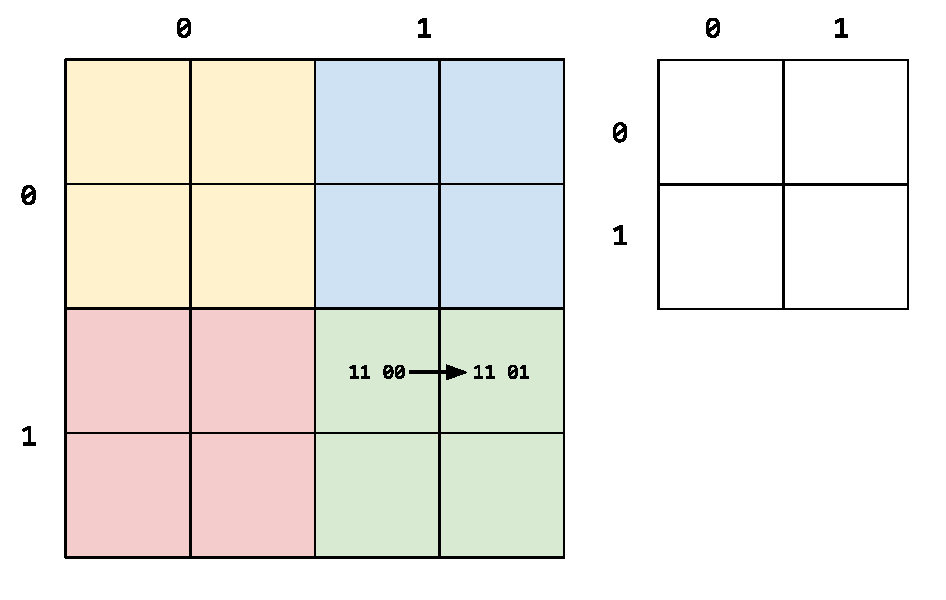
\includegraphics[width=8cm]{images/illustration-cpr-1.pdf}
\end{figure}

It is easy to see that the high 2 bits appeared in all positions, so we
can define a structure to do the following:

\begin{enumerate}
  \item The last two bits shall represent the local position
  \item The combination of first digit from two messages defines the higher grid
\end{enumerate}

Then the two messages can be sent as
\texttt{1\ 00\ -\textgreater{}\ 1\ 01}.

From lower bits \texttt{00\ -\textgreater{}\ 01}, we have four different
possibility of movement as shown in dashed arrows, and from the two
first bits combination \texttt{11}, we know that the arrow shall
represent the movement in the green grids:

\begin{figure}
  \center
  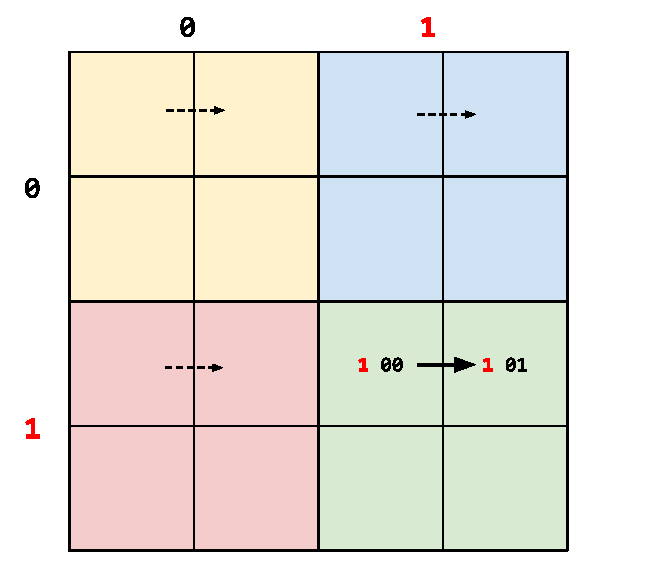
\includegraphics[width=5.5cm]{images/illustration-cpr-2.pdf}
\end{figure}

\subsection{The CPR and functions}\label{the-cpr-and-functions}

The actual CPR algorithm of course is more complicated, but the
principle is very similar to the previous example. If only one message
is given, it is possible to find multiple solutions that are spaced
around the world. The combination of two (different types of) messages
will yield the final result.

In CPR encoding, the Earth is divided in many zones (similar to the grid
in the previous example). And the encoding algorithm is also more
complicated (described in a later section). First, we will list some of
the parameters and common functions used in the decoding process here.

\subsubsection{NZ}\label{nz}

Number of geographic latitude zones between equator and a pole. It is
set to \texttt{NZ\ =\ 15} for Mode-S CPR encoding.

\subsubsection{floor(x)}\label{floorx}

the floor function \texttt{floor(x)} defines as the greatest integer
value k, such that \texttt{k\textless{}=x}, for example: :

\begin{verbatim}
floor(5.6) = 5
floor(-5.6) = -6
\end{verbatim}

\subsubsection{mod(x, y)}\label{modx-y}

the modulus function \texttt{mod(x,\ y)} returns:

\begin{equation}
  x - y \cdot floor(\frac{x}{y})
\end{equation}

where \texttt{y} can not be zero

\subsubsection{NL(lat)}\label{nllat}

Denotes the ``number of longitude zones'' function, given the latitude
angle \texttt{lat}. The returned integer value is constrained within
\texttt{{[}1,\ 59{]}}, calculated as:

\begin{equation}
  \text{NL}(lat) = floor \left( \frac{2 \pi}{\arccos(1 - \frac{1-\cos(\frac{\pi}{2 \cdot \text{NZ}})}{\cos^2(\frac{\pi}{180} \cdot \text{lat})}) } \right)
\end{equation}

For latitudes that are close to the equator or the poles, one of
following values is returned: :

\begin{verbatim}
lat = 0     ->    NL = 59
lat = +87   ->    NL = 2
lat = -87   ->    NL = 2
lat > +87   ->    NL = 1
lat < -87   ->    NL = 1
\end{verbatim}
